\section{Model Sequence to Sequence}
Model Sequence to Sequence (seq2seq) merupakan arsitektur Jaringan Saraf Berulang yang biasa digunakan untuk memecahkan masalah bahasa yang kompleks seperti Terjemahan, Menjawab Pertanyaan, membuat Chatbot, Peringkasan Teks, dll. Contoh penggunaan model seq2seq dapat dilihat pada gambar \ref{seqtoseq}
\begin{figure}[H]
        \centerline{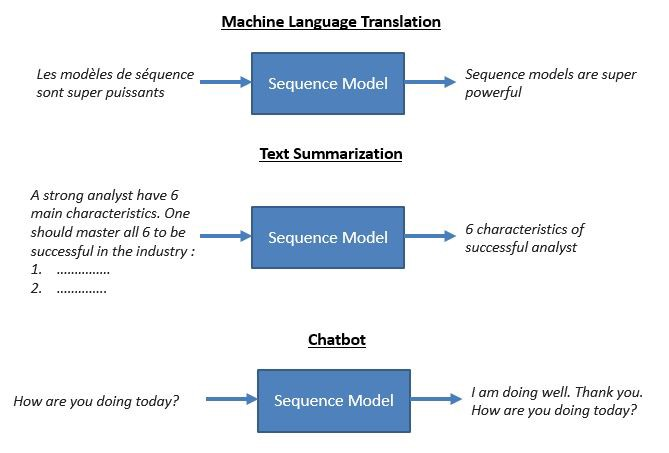
\includegraphics[scale=.45]{figures/sequence_model}}
        \caption{Contoh Penggunaan Model Sequence to Sequence}
		\label{seqtoseq}
\end{figure}

Model seq2seq sering dijumpai pada sistem yang sering kita gunakan sehari-hari. Model seq2seq mendukung aplikasi seperti Google Terjemahan, perangkat yang mendukung suara, voice assistant, chatbot, dll . Berikut ini adalah beberapa aplikasinya:

\begin{enumerate}
\item Google Translate, makalah tahun 2016 dari Google menunjukkan bagaimana kualitas terjemahan model seq2seq yang mendekati atau bahkan melampaui semua hasil yang dipublikasikan saat ini.
\begin{figure}[H]
        \centerline{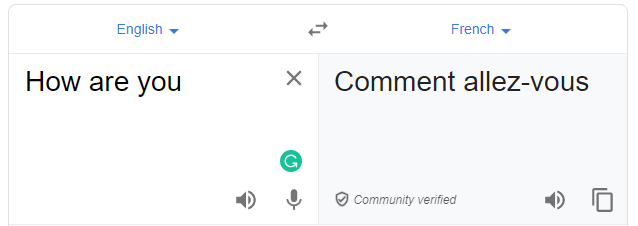
\includegraphics[scale=.5]{figures/terjemahan}}
        \caption{Google Translate}
		\label{terjemahan}
\end{figure}
\item Speech Recognition, makalah Google yang membandingkan model seq2seq yang ada pada pengenalan suara.
\begin{figure}[H]
        \centerline{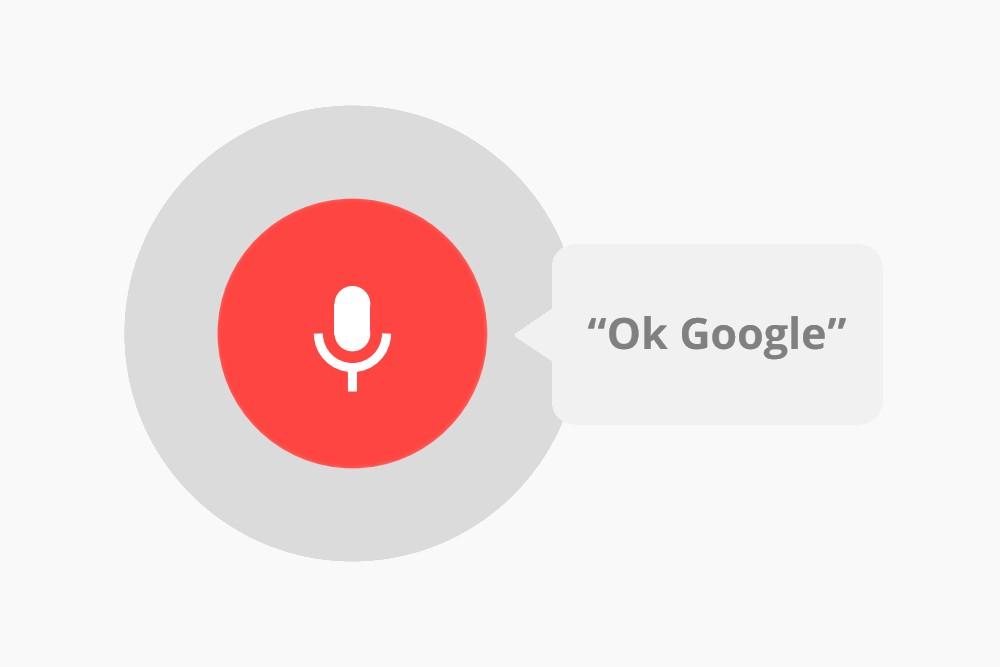
\includegraphics[scale=.25]{figures/voice}}
        \caption{Speech Recognition}
		\label{voice}
\end{figure}
\item Video Captioning –  Secara otomatis membuat subtitle video untuk setiap frame, termasuk deskripsi isyarat suara (seperti mesin yang dinyalakan, orang yang tertawa di latar belakang, dll.).
\begin{figure}[H]
        \centerline{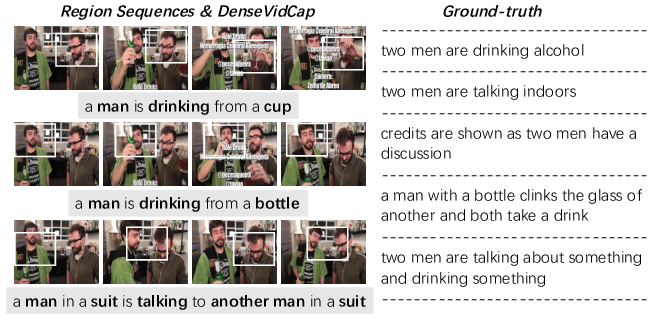
\includegraphics[scale=.45]{figures/video-captioning}}
        \caption{Video Captioning}
		\label{video}
\end{figure}
\end{enumerate}

Beberapa aplikasi tersebut membuat model seq2seq dipandang sebagai solusi terbaik. Model ini dapat digunakan sebagai solusi untuk setiap masalah berbasis urutan, terutama yang input dan outputnya memiliki ukuran dan kategori yang berbeda.

\subsection{Arsitektur Encoder-Decoder}
Arsitektur yang paling umum digunakan untuk membangun model Seq2Seq adalah arsitektur Encoder-Decoder.

Encoder:
\begin{enumerate}
\item Encoder dan decoder adalah model LSTM (atau terkadang model GRU)
\item Encoder membaca urutan input dan merangkum informasi dalam sesuatu yang disebut internal state vectors atau context vector (dalam kasus LSTM ini disebut hidden state dan cell state vectors). Kami membuang output encoder dan hanya mempertahankan status internal. Vektor konteks ini bertujuan untuk merangkum informasi untuk semua elemen input untuk membantu dekoder membuat prediksi yang akurat.
\item Hidden State h\_i dihitung menggunakan rumus pada gambar \ref{rumus}:
\begin{figure}[H]
        \centerline{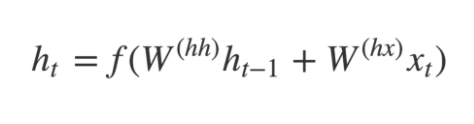
\includegraphics[scale=.3]{figures/rumus}}
        \caption{Rumus Hidden State}
		\label{rumus}
\end{figure}
\end{enumerate}

Perhatikan gambar \ref{encoder} LSTM membaca data dari satu urutan secara berurutan. Jadi jika inputnya adalah barisan dengan panjang 't', kita katakan bahwa LSTM membacanya dalam langkah waktu 't'.

\begin{figure}[H]
        \centerline{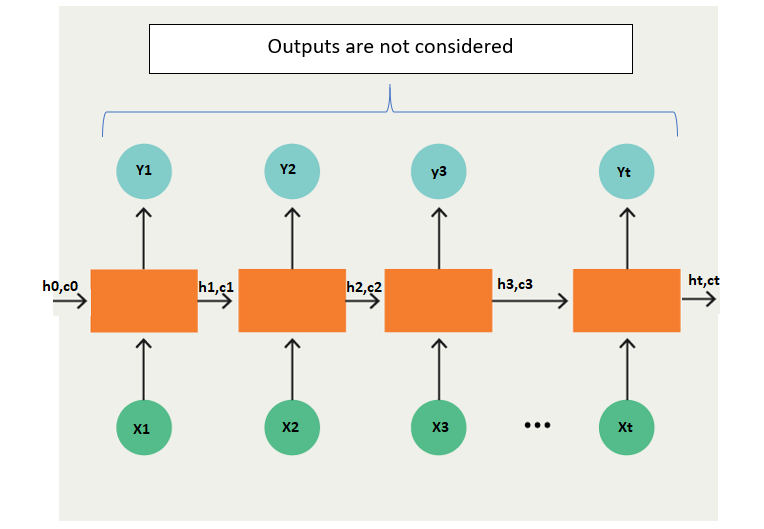
\includegraphics[scale=.45]{figures/lstm}}
        \caption{Encoder}
		\label{encoder}
\end{figure}

\begin{enumerate}
\item Xi = Urutan input pada langkah waktu i.
\item hi dan ci = LSTM mempertahankan dua status ('h' untuk status tersembunyi dan 'c' untuk status sel) pada setiap langkah waktu. h dan c yang dikombinasikan bersama-sama merupakan keadaan internal LSTM pada langkah waktu i.
\item Yi = Urutan keluaran pada langkah waktu i. Yi sebenarnya adalah distribusi probabilitas atas seluruh kosakata yang dihasilkan dengan menggunakan aktivasi softmax. Jadi setiap Yi adalah vektor dengan ukuran “vocab\_size” yang mewakili distribusi probabilitas.
\end{enumerate}

Dekoder:
\begin{enumerate}
\item Decoder adalah LSTM yang status awalnya diinisialisasi ke final state Encoder LSTM, yaitu context vector dari final cell encoder dimasukkan ke first cell pada jaringan decoder. Dengan menggunakan initial states ini, dekoder mulai menghasilkan output sequence, dan output ini juga dipertimbangkan untuk output selanjutnya.
\item Tumpukan beberapa unit LSTM di mana masing-masing memprediksi output y\_t pada langkah waktu t.
\item Setiap unit berulang menerima hidden state dari unit sebelumnya menghasilkan dan mengeluarkan hidden statenya sendiri.
\item Setiap hidden state h\_i dihitung menggunakan rumus:
\begin{figure}[H]
        \centerline{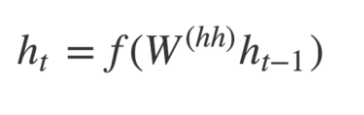
\includegraphics[scale=.3]{figures/rumus-encoder}}
        \caption{Rumus Hidden State}
		\label{rumus1}
\end{figure}
\item Output y\_t pada langkah waktu t dihitung dengan menggunakan rumus:
\begin{figure}[H]
        \centerline{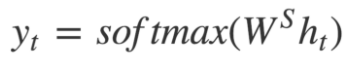
\includegraphics[scale=.3]{figures/rumus2}}
        \caption{Rumus Hidden State}
		\label{rumus2}
\end{figure}

Menghitung output dilakukan dengan menggunakan hidden state pada langkah waktu saat ini bersama-sama dengan respective weight W(S). Softmax digunakan untuk membuat vektor probabilitas yang akan membantu kita menentukan hasil akhir (misalnya kata dalam masalah tanya jawab).
\begin{figure}[H]
        \centerline{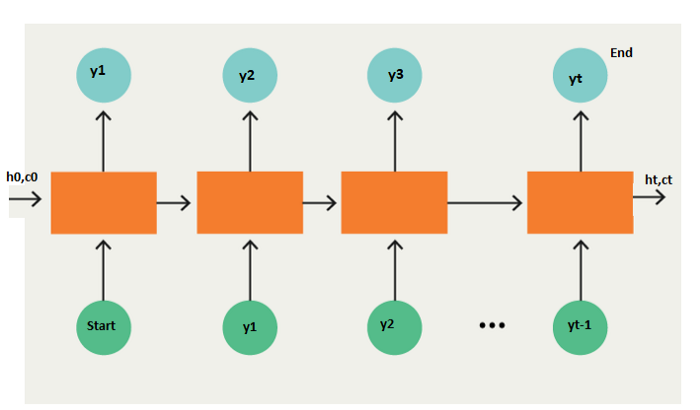
\includegraphics[scale=.45]{figures/lstm1}}
        \caption{Decoder}
		\label{decoder}
\end{figure}
\end{enumerate}

Sebagai contoh kita akan menambahkan dua token dalam urutan output sebagai berikut:

Contoh:
“ START\_ John pekerja keras \_END ”.

Poin yang paling penting adalah bahwa first state (h0, c0) dari dekoder diatur ke final state dari encoder. Ini secara intuitif berarti bahwa decoder dilatih untuk mulai menghasilkan urutan output tergantung pada informasi yang dikodekan oleh encoder. Sehingga loss dihitung pada output yang diprediksi dari setiap langkah waktu dan error disebarkan kembali melalui waktu untuk memperbarui parameter jaringan. Training network dalam jangka waktu yang lebih lama dengan jumlah data yang cukup besar menghasilkan prediksi yang cukup bagus.

\begin{figure}[H]
        \centerline{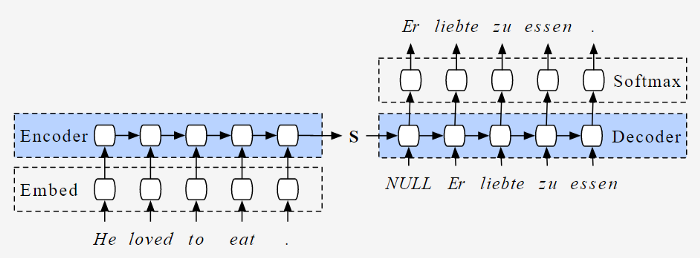
\includegraphics[scale=.45]{figures/arsitektur-encoder-decoder}}
        \caption{Arsitektur Encoder-Decoder Secara Keseluruhan}
		\label{endecoder}
\end{figure}

\begin{enumerate}
\item Selama inferensi dihasilkan satu kata pada satu waktu.
\item Initial state dekoder diatur ke final state encoder.
\item initial input ke dekoder selalu berupa token START.
\item Pada setiap time step kita harus mempertahankan status dekoder dan menetapkannya sebagai status awal untuk time step berikutnya.
\item Pada setiap time step, output yang diprediksi diumpankan sebagai input pada time step berikutnya.
\item loop akan dihentikan ketika decoder memprediksi token END.
\end{enumerate}

Sebuah sequence untuk model urutan memiliki dua bagian - encoder dan decoder.  Kedua bagian itu praktis adalah dua model jaringan saraf yang berbeda digabungkan menjadi satu jaringan raksasa. Secara umum, tugas jaringan encoder adalah memahami urutan input, dan membuat representasi dimensi yang lebih kecil darinya. Representasi ini kemudian diteruskan ke jaringan decoder yang menghasilkan urutannya sendiri yang mewakili output. Mari kita ambil contoh agen percakapan untuk memahami konsepnya.

\begin{figure}[H]
        \centerline{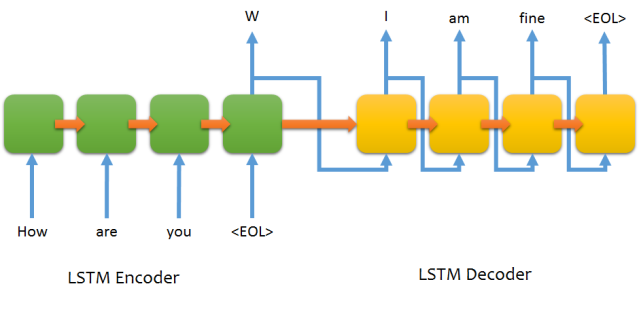
\includegraphics[scale=.65]{figures/chatbot}}
        \caption{Chatbot dengan Seq2Seq Model}
		\label{chatbot}
\end{figure}

Pada gambar \ref{chatbot}, urutan input adalah "Bagaimana kabarmu". Jadi ketika urutan input seperti itu dilewatkan melalui jaringan encoder-decoder yang terdiri dari blok LSTM (sejenis arsitektur RNN), decoder menghasilkan kata-kata satu per satu di setiap langkah waktu iterasi dekoder. Setelah satu iterasi penuh, urutan output yang dihasilkan adalah "Saya baik-baik saja".

\subsection{Kekurangan Model Encoder-Decoder}
Ada dua kelemahan utama arsitektur ini, keduanya terkait dengan panjang.

Pertama, seperti halnya manusia, arsitektur ini memiliki memori yang sangat terbatas. Keadaan tersembunyi terakhir dari LSTM, yang kami sebut S atau W , adalah saat Anda mencoba menjejalkan keseluruhan kalimat yang harus Anda terjemahkan. S atau W biasanya hanya beberapa ratus unit (baca: bilangan floating-point)  semakin Anda mencoba untuk memaksa ke dalam vektor dimensi tetap ini, semakin besar kerugian jaringan saraf yang dipaksakan. Memikirkan jaringan saraf dalam hal "kompresi lossy" yang harus mereka lakukan terkadang cukup berguna.
Kedua, sebagai aturan umum, semakin dalam jaringan saraf, semakin sulit untuk dilatih. Untuk jaringan saraf berulang, semakin panjang urutannya, semakin dalam jaringan saraf sepanjang dimensi waktu. Ini menghasilkan gradien yang hilang, di mana sinyal gradien dari tujuan yang dipelajari oleh jaringan saraf berulang menghilang saat bergerak mundur. Bahkan dengan RNN yang dibuat khusus untuk membantu mencegah gradien yang hilang, seperti LSTM, ini masih merupakan masalah mendasar.
Selanjutnya, untuk kalimat yang lebih kuat dan panjang, kami memiliki model seperti Attention Models dan Transformers . 

\subsection{Sequence to Sequence dengan Attention}
Deep Learning dalam skala besar mengganggu banyak industri dengan membuat chatbot dan bot yang belum pernah ada sebelumnya. Di sisi lain, seseorang yang baru memulai Deep Learning akan membaca tentang Dasar-dasar Neural Networks dan berbagai arsitekturnya seperti CNN dan RNN. Tapi sepertinya ada lompatan besar dari konsep sederhana ke aplikasi industri Deep Learning. Konsep-konsep seperti Batch Normalization, Dropout dan Attention hampir merupakan persyaratan untuk diketahui dalam membangun aplikasi deep learning. Berikut dua konsep penting yang digunakan dalam aplikasi terkini dalam Pengenalan Ucapan dan Pemrosesan Bahasa Alami – yaitu pemodelan Sequence to Sequence dan Attention Model. Sekadar memberikan gambaran tentang potensi penerapan kedua teknik ini Sistem AI Baidu menggunakannya untuk membuat kloningan suara manusia. Ini mereplikasi suara seseorang dengan memahami suaranya hanya dalam tiga detik pelatihan. Kita dapat melihat beberapa  sampel audio yang  disediakan oleh Tim Riset Baidu yang terdiri dari suara asli dan suara yang disintesis. Ketika manusia mencoba memahami sebuah gambar, ia memfokuskan pada bagian-bagian tertentu dari gambar untuk mendapatkan keseluruhan esensi dari gambar tersebut. Dengan cara yang sama, kita dapat melatih sistem buatan untuk fokus pada elemen tertentu dari gambar untuk mendapatkan keseluruhan "gambar". Ini pada dasarnya adalah bagaimana mekanisme perhatian bekerja. Mari kita ambil contoh masalah teks gambar, di mana sistem harus menghasilkan teks yang sesuai untuk gambar. Dalam skenario ini, untuk menghasilkan keterangan, mekanisme perhatian membantu model untuk memahami bagian-bagian individu dari gambar yang paling penting pada contoh tertentu. Perhatikan gambar \ref{gambar} 

\begin{figure}[H]
        \centerline{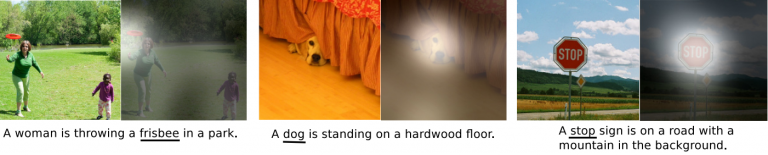
\includegraphics[scale=.5]{figures/gambar3}}
        \caption{Gambar to Text}
		\label{gambar}
\end{figure}

Untuk menerapkan mekanisme attention, kami mengambil input dari setiap langkah waktu encoder tetapi memberi bobot pada langkah waktu. Pembobotan tergantung pada pentingnya langkah waktu tersebut bagi dekoder untuk menghasilkan kata berikutnya secara optimal dalam urutan, seperti yang ditunjukkan pada gambar \ref{attention}

\begin{figure}[H]
        \centerline{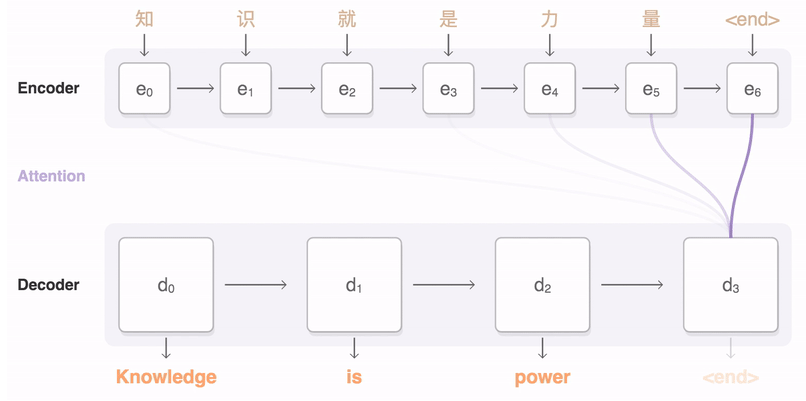
\includegraphics[scale=.5]{figures/gambar1}}
        \caption{Mekanisme Attention pada Gambar to Text}
		\label{attention}
\end{figure}


\subsection{Rumusan Masalah untuk Pemodelan Sequence to Sequence}
Kita tahu bahwa untuk memecahkan masalah pemodelan sequence, Jaringan Syaraf Tiruan adalah arsitektur terbaik yang dapat kita pilih. Mari kita ambil contoh Sistem Penjawab Pertanyaan untuk memahami seperti apa masalah pemodelan urutan. Misalkan terdapat serangkaian pernyataan sebagai berikut:

Jo pergi ke dapur. Fred pergi ke dapur. Joe mengambil susu itu.

Joe pergi ke kantor. Joe meninggalkan susu. Jo pergi ke kamar mandi.

Pertanyaannya dimana joe sebelum pergi ke kantor? Jawaban yang tepat adalah "dapur". Pandangan sekilas membuat ini tampak seperti masalah sederhana. Tetapi untuk memahami kompleksitasnya terdapat dua dimensi yang harus dipahami oleh sistem:

\begin{enumerate}
\item Pemahaman dalam bahasa Inggris dan urutan karakter/kata yang membentuk kalimat.
\item Urutan peristiwa yang berkisar pada orang-orang yang disebutkan dalam pernyataan.
\end{enumerate}
Ini dapat dianggap sebagai masalah pemodelan urutan, karena memahami urutan itu penting untuk membuat prediksi apa pun di sekitarnya. Ada banyak skenario masalah pemodelan urutan seperti itu, yang dirangkum dalam gambar di bawah ini. Contoh yang diberikan di atas adalah masalah banyak inputan dengan satu output (Jika Anda menganggap sebuah kata sebagai output tunggal).
